\documentclass[a4paper,10pt]{article}
\usepackage[utf8]{inputenc}
\usepackage[frenchb]{babel}
\usepackage[T1]{fontenc}

%%%%%%%%%%%%%%%%%%%%%%%%%%%%%%%%%%%%%%
\usepackage{calc}
\usepackage{ifthen}
\usepackage{tikz}
\newcommand{\slice}[4]{
  \pgfmathparse{0.5*#1+0.5*#2}
  \let\midangle\pgfmathresult

  % slice
  \draw[thick,fill=black!10] (0,0) -- (#1:1) arc (#1:#2:1) -- cycle;

  % outer label
  \node[label=\midangle:#4] at (\midangle:1) {};

  % inner label
  \pgfmathparse{min((#2-#1-10)/110*(-0.3),0)}
  \let\temp\pgfmathresult
  \pgfmathparse{max(\temp,-0.5) + 0.8}
  \let\innerpos\pgfmathresult
  \node at (\midangle:\innerpos) {};
}
%%%%%%%%%%%%%%%%%%%%%%%%%%%%%%%%%%%%%%

\usepackage{authblk}
\usepackage{frbib}
\usepackage{amsfonts}
\usepackage{amsmath}
\usepackage{amssymb}
\usepackage{array}
\usepackage{url}
\usepackage{hyperref}
\usepackage{textcomp}
\usepackage[all]{hypcap}
\usepackage[labelseparator=endash]{caption}
\usepackage[listofformat=parens]{subfig}
\usepackage{graphicx, color}
\usepackage{listings}
\usepackage{float}
\bibliographystyle{frplain}
\hypersetup{colorlinks,%
            citecolor=black,%
            filecolor=black,%
            linkcolor=black,%
            urlcolor=blue}

\newcommand{\LSTRESET}{
  \lstset{
    language=,
    basicstyle=\color{black},
    identifierstyle=\color{black}
}
}


\setlength{\affilsep}{0.2cm}
\author{Thomas Coursin, Ken Déguernel, François Deslandes}
\affil{Génie Mathématique 5ème année}
\affil{A l'attention de Mme Lehmann}
%\date{4 Décembre 2013\\}
\title{\Huge{Entrée en bourse des réseaux sociaux}\\
\LARGE{Etude comparative Facebook vs. Twitter}\\
\vspace{10mm}
}

\DeclareMathOperator{\Rec}{Rec}
\DeclareMathOperator{\card}{card}

\begin{document}
\maketitle\thispagestyle{empty}
 
\newpage\null\thispagestyle{empty}\setcounter{page}{0}

\tableofcontents

\clearpage

% ARTICLES
% http://www.lemonde.fr/technologies/article/2013/11/07/twitter-entre-en-bourse-jeudi-a-26-dollars-par-action_3509501_651865.html
% http://www.lemonde.fr/technologies/article/2012/05/24/entree-en-bourse-de-facebook-les-raisons-d-un-fiasco_1706425_651865.html
% http://www.lemonde.fr/technologies/article/2013/11/06/l-entree-en-bourse-de-twitter-s-accompagne-d-un-parfum-de-bulle-financie_3509075_651865.html
% http://www.lemonde.fr/technologies/article/2014/02/06/twitter-creuse-ses-pertes-depuis-son-introduction-en-bourse_4361327_651865.html


\section{Introduction}

L'entrée en bourse des réseaux sociaux est un nouveau cas d'étude en finance. De nombreuses interrogations ont accompagné les entrées en bourse de Twitter et de Facebook pour plusieurs raisons.
D'abord parce que ces entreprises sont basées sur des modèles économiques qui doivent faire leurs preuves. Ces deux entreprises doivent montrer aux marchés financiers qu'elles sont capables de monétiser les investissements.
Les marchés financiers attendent aussi de Facebook et Twitter qu'ils soient capable de s'inscrire dans le long terme en supportant des projets innovants capables de garantir la pérennité des investissements.
Enfin les entrées en bourses de Twitter et Facebook présentent de nombreux points de comparaison à la fois sur les choix de chaque entreprises et sur la réaction des marchés.


Dans la suite, nous allons présenter les deux réseaux sociaux, leurs modèles économiques et leurs actualités. Nous discuterons ensuite des choix relatifs à l'entrée en bourse et de la réaction des marchés. Ensuite nous effectuerons une comparaison des stratégies d'entrées en bourse. Enfin, nous évoquerons la vie des titres et les attentes des marchés financiers.

\vspace{1cm}
\begin{center}

\includegraphics[scale=0.3]{./images/facebook_vs_twitter.png}
\end{center}

\newpage
\section{Présentations}
Le terme de réseau social désigne un site internet permettant de se constituer un réseau d'amis ou de connaissances avec lesquels ont peut communiquer par le biais d'un certain nombre d'outils de communication.


% Présentation générale des deux réseaux sociaux :
% Utilisateurs, Business model, Management.
% Leur actualité :
% Concurrent, nouveautés (facebook on mobile), débat sur la confidentialité des données, etc.
% résultats

\subsection{Facebook}
Facebook est le premier réseau social du monde avec 1.9 millards d'utilisateurs actifs par mois. La majeure partie de ces utilisateurs sont localisés en Amérique du Nord. Les utilisateurs de Facebook sont d'origines variées et regroupent des utilisateurs classiques, des développeurs et des publicitaires.


Créé en 2004 par Marc Zuckerberg, Facebook était un site destiné aux étudiants de la faculté d'Harvard. Suite au succès de la plateforme, Facebook s'est développé et est maintenant disponible partout dans le monde. Facebook permet à ses utilisateurs d'entrer des informations personnelles et d’interagir avec d'autres utilisateurs. Ce réseau social est principalement basé sur le concept d'amitié. Il est possible de partager du contenu avec un groupe restreint de personnes appelés "amis".
Les possibilité offertes par le réseau social se sont largement diversifiée et il est maintenant possible d'organiser ses contacts en groupes (amis, collègues, etc) et même de jouer à des jeux.



\subsection{Twitter}

Twitter est le second réseau social dans le monde et principal concurrent de Facebook avec 240 millions d'utilisateurs par mois dans le monde. A la différence de Facebook, 77\% de ses utilisateurs se situe en dehors de l’Amérique du nord. Ses utilisateurs sont des utilisateurs classiques, des développeurs ou des entreprises.

Créé en 2006 par Jack Dorsey, le service est basé sur l'échange de messages brefs consultables par tous les utilisateurs. Les utilisateurs peuvent "suivre" d'autres utilisateurs, ce qui leur permet de recevoir directement les messages publiés sur leur "timeline", c'est-à-dire leur page principale. Contrairement à Facebook, Twitter souhaite garder une utilisation simple qui a peu changé depuis sa création.

Twitter est très utilisés par les personnalités, les politiques qui s'en servent pour faire passer des annonces voire même en lieu et place de communiqués de presse. Ces messages sont très souvent relayés par les médias.


\subsection{Financement}

L'inscription et l'utilisation de Facebook et de Twitter est entièrement gratuite. L'une des sources de revenue évidente est la publicité.

Facebook se finance en grande partie par la publicité ciblée basée sur les profils des utilisateurs. La Publicité vidéo a fait son apparition sur Facebook qui en attend des revenus proches de 4 millions de dollars par jour.

Twitter, en revanche,concentre sa stratégie sur l'augmentation de son nombre d'utilisateurs. Des publicités ciblées existent malgré tout sur Twitter et sont intégrées directement à l'environnement et passent donc presque inaperçu. Twitter se finance principalement par des appels publics à l'épargne auprès de fonds d’investissements.

\subsection{Achats d'entreprises}

Facebook souhaite renforcer sa position sur le marché des réseaux sociaux. C'est dans cette démarche que le réseau social N°1 rachète des entreprises concurrente. On peut noter notamment le rachat d'Instagram en 2012, l'application de partage de photos, pour une somme de 1 milliard de dollars jugée trop élevée pour une entreprise qui ne rapporte rien. Ce rachat est expliqué par la volonté de Facebook d’asseoir sa position de leader et de combler ses manques au niveau du partage de photos sur mobile.
Facebook a aussi racheté Whatsapp en 2014, une application d'échange de messages sans opérateur, pour 19 milliards de dollars. Avec ce rachat, perçu comme une démonstration de force, Facebook veut clairement montrer son envie de conserver sa place de leader.


Twitter est beaucoup plus discret sur le rachat d'entreprises et on peut noter seulement le rachat de Tweetdeck en 2011, une application basée sur Twitter proposant une interface conviviale.

\section{Entrée en bourse}
% Nombre d'action, répartition, prix, controle, facteurs de risque
% Entrée en bourse, réaction, faits marquants
% Evolution consécutive

\subsection{Facebook}
Lors de son entrée à la bourse de New York, Facebook crée deux types d'action. Des actions de Classe A correspondant à une voix, et des actions de Classe B correspondant à dix voix. Facebook proposa en première offre publique 421.233.615 actions de classe A au prix de 38\$ l'unité. Ces actions sont constituées de 180.000.000 nouvelles actions et de 241.233.615 actions provenant d'actionnaires vendeurs.\\
Le prix élevé des actions est justifié par la position de leader de Facebook 
et par des antécédents financiers robuste. Juste après la première offre publique, le prix moyen d'action recherché par les traders est 34,7\$.\\

Le système mis en place avec deux classes d'actions permet à Mark Zuckerberg de garder un contrôle majoritaire sur Facebook.
Après la première offre publique, on a :
\[
\begin{array}{c|c}
	\text{Possession d'action} & \text{Votes}\\
	\hline
	\begin{tikzpicture}[scale=1.2]
\newcounter{a}
\newcounter{b}
\foreach \p/\t in {33/Zuckerberg, 33/Autres dirigeants, 34/Flottant}
  {
    \setcounter{a}{\value{b}}
    \addtocounter{b}{\p}
    \slice{\thea/100*360}
          {\theb/100*360}
          {\p\%}{\t}
  }
	\end{tikzpicture}
	&
	\begin{tikzpicture}[scale=1.2]
\foreach \p/\t in {60/Zuckerberg, 35/Autres dirigeants, 5/Flottant}
  {
    \setcounter{a}{\value{b}}
    \addtocounter{b}{\p}
    \slice{\thea/100*360}
          {\theb/100*360}
          {\p\%}{\t}
  }
	\end{tikzpicture}
\end{array}
\]
\\

Cependant, Facebook possède plusieurs facteurs de risque :
\begin{itemize}
\item son business model est très dépendant de la publicité,
\item sa capacité à conserver son nombre utilisateur actif peut être mit en question,
\item sa capacité à gérer la compétition grandissante,
\item sa capacité de monétiser les investissement est encore à prouver,
\item les mesures prises par le gouvernement sur la sécurité de l'information et sur la protection de la vie privée peuvent limiter les possibilités de Facebook d'un point de vue légal.\\
\end{itemize}

Le premier jour, le prix de l'action n'a augmenté que de 10\%. Grâce au support des banques d'investissements, le premier prix de fermeture fut proche de celui proposé (38,23\$). Dans les jours suivants, le prix de l'action baisse drastiquement jusqu'à 28,19\$.\\
\begin{center}
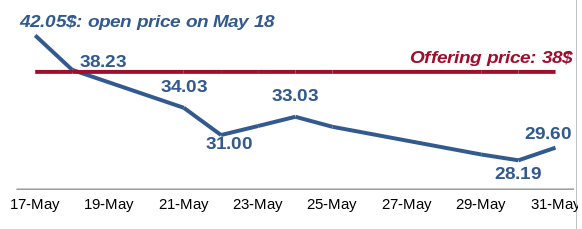
\includegraphics[scale=0.4]{images/FBIPO.png}
\end{center}

Cela peut s'expliquer par plusieurs facteurs extérieurs:
\begin{itemize}
\item des problèmes techniques du Nasdaq ont retardé l'affichage de la cote de 30 minutes,
\item la Federal Trade Commission a commencé une enquête sur le rachat d'Instagram par Facebook en mai,
\item General Motors a annoncé qu'il ne publierai plus de publicité sur Facebook,
\item des investisseurs ont mit Mark Zuckerberg en procès par rapport à la première offre publique, considérée comme injuste envers les actionnaires.
\end{itemize}
Ce phénomène peut aussi s'expliquer par des erreurs de management :
\begin{itemize}
\item prise de risque en mettant un prix d'action élevé,
\item mauvais timing d'entrée sur le marché. Les conditions du marché étaient mauvaises (l'indice S\&P500 venait de baisser de 7\%).\\
\end{itemize}

Suite à la première offre publique, les actions suivent le mouvement suivant :
\begin{center}
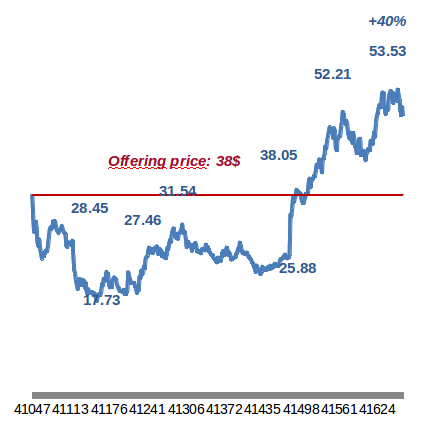
\includegraphics[scale=0.4]{images/FBpostIPO.png}
\end{center}
Tout d'abord, les actions atteignent le prix minimum 17,73\$ par action. Ceci entraînant des revenus décevants.\\
Début Août 2013, le prix des actions augmente de 40\%. Cela entraîne des revenues supérieurs à ceux prévus (+53\%), et une grande augmentation du taux de pénétration sur le marché du mobile.\\
Depuis, les actions subissent une augmentation constante suite à une grande croissance en 2013 (revenus provenant des mobiles multipliés par 3). Le 24 Mars 2014, les actions Facebook ont pour prix de clôture 64,1\$.

\subsection{Twitter}
Lors de son entrée à la bourse de New York, Twitter propose en première offre publique 70.000.000 d'actions (de même classe) au prix de 26\$ par action. Il s'agit uniquement de nouvelles actions.
Suite à la première offre publique, les nouveaux actionnaires représentent 12,8\% du capital.
Après la première offre publique, on a :
\[
\begin{array}{c|c}
	\text{Possession d'action} & \text{Votes}\\
	\hline
	\begin{tikzpicture}[scale=1.2]
\foreach \p/\t in {87/Flottant, 13/Dirigeants}
  {
    \setcounter{a}{\value{b}}
    \addtocounter{b}{\p}
    \slice{\thea/100*360}
          {\theb/100*360}
          {\p\%}{\t}
  }
	\end{tikzpicture}
	&
	\begin{tikzpicture}[scale=1.2]
\foreach \p/\t in {87/Flottant, 13/Dirigeants}
  {
    \setcounter{a}{\value{b}}
    \addtocounter{b}{\p}
    \slice{\thea/100*360}
          {\theb/100*360}
          {\p\%}{\t}
  }
	\end{tikzpicture}
\end{array}
\]
\\
Twitter possède également plusieurs facteurs de risque :
\begin{itemize}
\item son business model est très dépendant de la publicité,
\item sa capacité à conserver son nombre utilisateur actif peut-être mit en question,
\item sa capacité à gérer la compétition grandissante,
\item aucun profit n'a été fait.
\\
\end{itemize}

Le premier jour, le prix de clôture des actions Twitter atteint 45\$ (soit une augmentation de 80\%). Depuis, le prix des actions est resté fort, jusqu'à atteindre 73\$.\\

\begin{center}
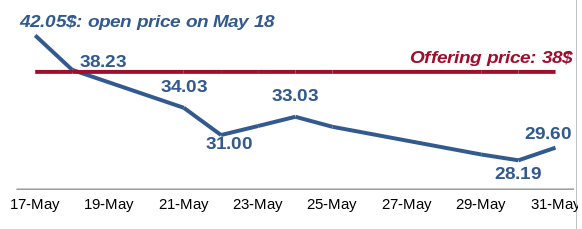
\includegraphics[scale=0.4]{images/FBIPO.png}
\end{center}

Cela peut s'expliquer par le fait que Twitter a évité la plupart des erreurs de Facebook :
\begin{itemize}
\item pas de vente d'actions déjà existante,
\item un nombre d'action limité : seulement 13\% de nouvelles actions, entraînant une demande dix fois supérieur au nombre d'actions offertes,
\item le nombre d'action offert est resté constant,
\item la première offre publique a eu lieu seulement un mois après l'annonce de la mise en bourse (contre trois mois pour Facebook),
\item un prix d'action assez faible permettant de réévaluer les actions à la hausse,
\item pas de difficulté technique lors de la première offre publique.
\end{itemize}

Au 24 Mars 2014, les actions Twitter ont pour prix de clôture 48.77\$.

\section{Conclusion}
% Twitter n'a pas commis les erreurs de Facebook
% Parler des stratégies (prix, répartition et vente des actions)
% Cas d'étude intéressant pour l'avenir avec la possible entrée en bourse de nouvelle entreprises simialaires ?????

\section{Vie des titres}
% Facebook qui monte
% Twitter qui baisse
% Possibilité de bulle financière
% Autres entrées en bourses de société de nouvellles technologies


\clearpage
\end{document}